\section{Pokemon mechanics}
\label{sec:pokemon-mechanics}

The Pokemon games are home to a vast amount of mechanics. In order to fully understand
this project, it is important to have a basic understanding of the mechanics present in a Pokemon battle.

The following section aims to briefly explain these mechanics.

\subsection{Type chart}
A Pokemon will under normal circumstances have 1 or 2 types that represents its elemental alignment and similarly a Pokemon move will have 1 type.
Each type determines its effectiveness against other types. The effectivenesses are categorized as follows:
\begin{itemize}
  \item No effect (0x multiplier)
  \item Not very effective (0.5x multiplier)
  \item Effective (1x multiplier)
  \item Super effective (2x multiplier)
\end{itemize}
These multipliers are stacking, so if a Pokemon has 2 types that resists an incoming attack, the multiplier becomes $ 0.5*0.5=0.25 $.
\notebox{Example: A fire type Pokemon, Charmander, is in a battle with the water type Pokemon, Squirtle.
  The Squirtle uses the water type move Water Gun against the Charmander. As water is super effective against fire, the move
  Water Gun receives a 2x multiplier to its damage.}

For the full list of type advantages and disadvantages, see appendix \ref{appendix:type-chart}.

\subsection{Stats}
A Pokemons power is determined by its stats. Since generation 2 a Pokemon has been described by the following stats:
\begin{itemize}
  \item HP: Determines the amount of hit points a Pokemon has. The more hit points a Pokemon has, the more durable it is.
  \item Attack: Determines the power of physical attacking moves.
  \item Defense: Determines a Pokemons resistance to physical attacking moves.
  \item Special Attack: Determines the power of special attacking moves.
  \item Special Defense: Determines a Pokemons resistance to special attacking moves.
  \item Speed: Determines a Pokemons speed, which is used to determine who goes first in a round of battle.
\end{itemize}
A Pokemons stats are influenced by a few factors: its base stats, level, nature, individual values and effort values.
Together they compose the Pokemons actual stats.

\subsubsection{IVs and EVs}
Individual values \cite{IndividualValues} and effort values \cite{EffortValues} (referred to as IVs and EVs) are hidden values attributed to a Pokemon to create variety in each Pokemons power levels within its species.
When a Pokemon is encountered it will be generated with IVs ranging from 0-31 for each of its stats. A higher IV will result in a higher total stat.

EVs are values gained through battles. A Pokemon can have a total number of 510 EVs with a limit of 255 points per stat.

\subsubsection{Natures}
A Pokemons nature \cite{Natures} is determined when it is generated. A nature gives a Pokemon a ±10\% modifier to select stats.
If a nature both raises and lowers a stat it is called a "Neutral nature" and no changes will occur to the final stat.
Please refer to figure \ref{tab:nature-table} for the full list of natures and their effects.
\begin{figure}[h]
  \centering
  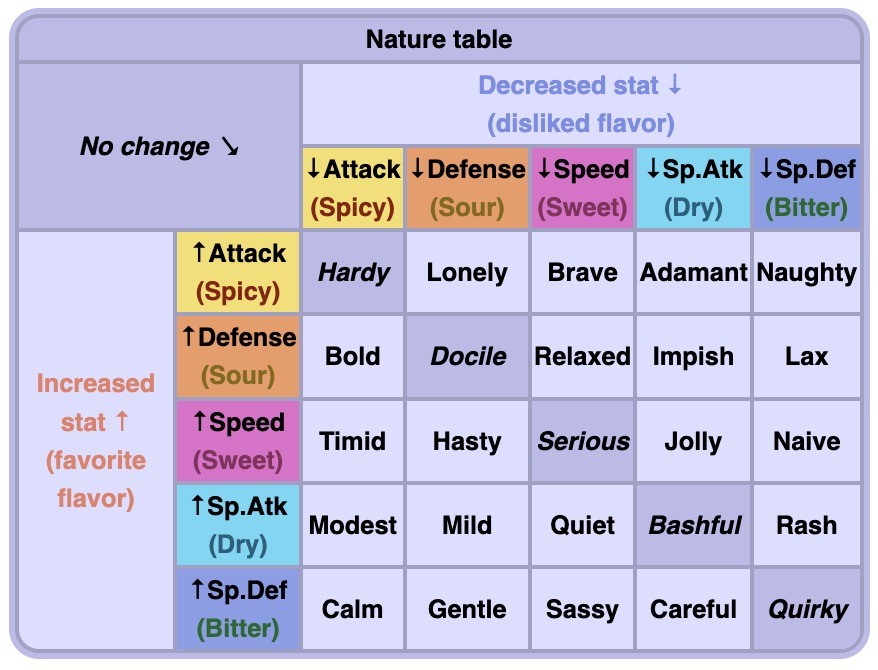
\includegraphics[width=.8\textwidth]{assets/nature-stat-table.jpg}
  \caption{Table of Natures and how they affect stats from Bulbapedia \cite{Natures}}
  \label{tab:nature-table}
\end{figure}

\subsubsection{Stat boosts}
Stat boosts are temporary modifiers applied to a Pokemons stat in combat. A stat is raised and lowered in stages ranging from -6 to +6 \cite{StatBoosts}.
Certain moves or abilities can raise or lower a Pokemons stat in stages. By default all stats begin at stage 0, meaning no change.

\begin{figure}[h]
  \centering
  \scalebox{.8}{
    \begin{tabular}{|c|c|c|c|c|c|c|c|c|c|c|c|c|c|}
      \hline
      \textbf{Stage}    & -6    & -5    & -4    & -3    & -2    & -1    & 0     & +1    & +2    & +3    & +4    & +5    & +6    \\
      \hline
      \textbf{Modifier} & $2/8$ & $2/7$ & $2/6$ & $2/5$ & $2/4$ & $2/3$ & $2/2$ & $3/2$ & $4/2$ & $5/2$ & $6/2$ & $7/2$ & $8/2$ \\
      \hline
    \end{tabular}
  }
  \caption{Table of stat stages and their modifier from Bulbapedia \cite{StatBoosts}}
  \label{tab:stat-stage-modifiers}

\end{figure}

\subsubsection{Formula}
With the above sections in mind, the final stat value of a Pokemon can be calculated using the following formulas \cite{PokemonStats}.
Please note that the HP stat has a different formula compared to the other stats.

\begin{figure}
  $$
    HP = \left\lfloor \frac{(2 * Base + IV + \left\lfloor \frac{EV}{4} \right\rfloor) * Level}{100} \right\rfloor + Level + 10
  $$
  
  $$
    OtherStat = \left\lfloor \left( \left\lfloor \frac{(2 * Base + IV + \left\lfloor \frac{EV}{4} \right\rfloor) * Level}{100} \right\rfloor + 5 \right) * NatureMod \right\rfloor
  $$
  \caption{Formulas for calculating a Pokemons stats \cite{PokemonStats}}
  \label{formula:stat-formula}
\end{figure}

\subsection{Abilities}
\label{subsec:abilities}
Since generation 3 of Pokemon, a Pokemon has had an Ability \cite{Abilities}. These are passive effects that provide bonuses in battle or in the overworld.
A Pokemon species can have multiple possible abilities, but a single Pokemon will only ever have one that is determined when the Pokemon is generated.
Abilities can have a wide variety of effects, ranging from setting a weather condition upon entering battle \cite{DrizzleAbility}, to increasing the damage of certain types of moves \cite{IronFistAbility}.

There are almost 300 abilities available in generation 9 of Pokemon. For this project to accurately describe the real world, most of these should be implemented, but the focus will be to implement the most common ones.

\subsection{Held items}
A Pokemon is able to hold an item \cite{HeldItems}. These items provide an effect to the Pokemon that can significantly change how a battle pans out. Like Abilities (see \ref{subsec:abilities}),
held items can have a lot of different effects. Notable examples are berries that a Pokemon may consume during battle, such as a Sitrus Berry \cite{SitrusBerry} that a Pokemon will automatically eat
when its HP is reduced below 50\%, resulting in the Pokemon restoring 25\% of its maximum HP. There are also items that provide a bonus through the entire battle such as Choice Band \cite{ChoiceBand}.
The Choice Band increases the Pokemons Attack stat by 50\%, but only allows it to use the first move it selects. The effect resets when it is withdrawn from battle.

There are a \textit{lot} of held items in generation 9 of Pokemon. For this project, the focus will be to implement the most common ones and expanding the available selection of held items as the time frame allows. 

\subsection{Status conditions}
In pokemon there exists a variety of status conditions that fall into either of two categories: Volatile and Non-volatile. Non-volatile status conditions
lasts until a pokemon is healed, and volatile conditions only lasts for the duration of a battle. \cite{StatusCondition}
\begin{itemize}
  \item Poison (PSN): Is a condition non-volatile that deals 1/8 of the pokemon's health at the end of each turn and can only be avoided by a few abilities,
  moves or items.
  \begin{itemize}
    \item Badly Poisoned: Is another type of the non-volatile poison status condition that starts to deal 1/16 at the start of a turn, 
      but increases the damage taken by 1/16 every turn, so after 3 turns it deals 3/16 of a pokemons health. 
      This condition can be avoided by the same abilities, moves or items as the normal poison condition.
  \end{itemize}
  \item Burn (BRN): Is another non-volatile status condition that deals 1/16 from generation 1 and 7 onwards while also cutting the pokemons attack stat
    in half until the pokemon is heald. There are one ability and move that negates the attack drop from burn and turns it into an attack boost instead.
  \item Sleep (SLP): This condition causes a pokemon unable to use moves, except snore and sleep talk and 
    randomly lasts 1 to 3 turns in generation 5 and onwards. The first turn of sleep is always skipped.
  \item Paralysis (PAR): Is a non-volatile status condition that has a 25\% chance of preventing the pokemon from moving each turn and reduces a pokemons
    speed 50\% from generation 7 onwards.
  \item Freeze (FRZ): This is a non-volatile condition that renders the pokemon unable to move unless, it thawes out by a 20\% chance or 
    by using a move to thaw it out.
  \item Confusion: Is a type of volatile status condition that has a 33\% chance of causing a pokemon to hurt itself in its confusion instead of executing
    a selected move.
  \item Flinch: The flinch status is volatile and prevents an oppossing pokemon from moving for the turn it was flinched. This can be done by moves like 
    fake out that has Priority +3, and rock slide that has a 30\% chance of flinching if you move before the oppossing pokemon.
  \item Others: There are a lot of other volatile status conditions that are not as common as the ones mentioned above.
  \begin{itemize}
    \item Grounded: Pokemon that are grounded looses their imunity to ground type moves.
    \item Nightmare: Only affects sleeping pokemon and deal 1/4 of their hp each turn they stay asleep.
    \item Curse: Deals 1/4 of the users hp each turn if used by a ghost type. If not lowers the users speed by 1 stage and increases 
      the users attack and defense by 1 stage.
  \end{itemize}
\end{itemize}
\subsection{Moves}
% Power
% Damage range
% OHKO
% Critical hits
% Physical/Special
% Accuracy
% Priority
% Targeting
\subsection{Weather}
Weather in pokemon is a mechanic that changes the rules of the battle field. There exists 8 different types of weather: \cite{Weather}
\begin{itemize}
  \item Harsh Sunlight: Can be set up by the move Sunny day or the ability Drought. It boosts the power of fire type moves by 50\% and weakens 
    water type moves by 50\%. no pokemon can get the Frozen condition and makes the moves Solar Beam and Solar Blade only take 1 turn to charge.
  \item Rain: Is gives opposite boosts and weaknesses of Harsh Sunlight and can be set up by the move Rain dance or the ability Drizzle. It also makes moves
    like Thunder and Hurricane have 100\% accuracy.
  \item Hail/Snow: Hail got changed to the Snow weather in generation 8 and used to deal 1/16 of a pokemons health at the end of each turn if they werent ice 
    type. The newer Snow weather had the damage removed but instead gives ice types a 50\% increase in defense. It also makes the move blizzard by 
    pass accuarcy checks.
  \item Sandstorm: Works a lot like Hail/Snow, it damages all pokemon expect rock, ground and steel types for 1/16 of their health at the end of the turn. 
    Sandstorm also boosts the special defense of rock types by 50\% and is setup by the move sandstorm or by the ability Sand stream.
  \item Fog: Is a weather condition that only existed in the generation 4 games and Legends Arceus. it reduced the Accuracy of all moves, 
    and could only be removed by the move Defog, that also removes entry hazards and screen effects.
  \item Extremly Harsh Sunlight: Is a stronger version of Harsh Sunlight and can only appear by using Primal Groudon. This weather conditions makes any 
    water type move unusable while still giving fire type moves a boost in power. 
  \item Heavy Rain: Is the stronger version of rain and can only appear by using Primal Kyogre. This weather condition makes any fire type move unusable 
    while still giving water type moves a boost in power.
  \item Strong Winds: Is a weather condition unique to Mega Rayquaza and makes any move super effective move on flying types deal neutral damage instead.
\end{itemize}


\subsection{Terrain effects}
Terrain is one of the newer mechaincs in pokemon and was introduced in generation 7. There exists 4 different types of terrain and a variety of moves and abilities
that recieves a boost from having a terrain or remove terrain effects. Each Terrain lasts for 5 turns and can be overwritten by other terrains. \cite{Terrain}
\begin{itemize}
  \item Electric Terrain: Prevents all pokemon on the ground from falling asleep and boosts the power of electric type moves by 30\%.
  \item Grassy Terrain: Restores all grounded pokemon on the field by 1/16 of their max hp each turn and boosts the power of grass type moves by 30\%.
  \item Misty Terrain: Halves the damage taken from dragon type moves and prevents grounded pokemon from being affected by non-volatile status conditions and 
    confusion.
  \item psychic Terrain: Prevents pokemon on the ground from being hit by moves with increased priority, and boosts the power of psychic type moves by 30\%.
\end{itemize}

\subsection{Battles}
% Turn order
There exists a lot of different types of battles in the Pokemon games, the most common ones being Single battles and Double battles that have been present 
since generation 3. Each variation of battles builds upon the standard Single battle format. Single battles have 4 commands that can be done each turn:
\cite{PokemonBattles}
\begin{itemize}
  \item Battle: The player chooses a move to use against the opponent
  \item Pokemon: The player can switch to any pokemon in their party 
  \item Bag: The player can use items and berryies to heal their pokemon, this choice cannot be used in competitive battles.
  \item Run: The player can choose to run from a wild battle, but this choice cannot be used in trainer battles.
\end{itemize}
\subsubsection{Double battles}
Double battles are the main variation of the standard single battle format and is also the standard competitive format. In double battles 
each player sends out 2 pokemon at the start of the battle and can target any of the 4 pokemon on the field with their moves. Several moves change 
when used in a double battle, because they can be used to target both opponents, everyone except itself on the field or redirect moves.
This format gives a pokemon battle a lot more complexity and strategy than the single battle format, which is why it became the competitive standard.
Double battles also feature a mechanic that the single battle format doesnt have, a Dynamic turn order, which means that during a turn the pokemon
moving first can change during the turn. An example of having a dynamic turn order is with the move Tailwind tht doubles the speed of the users team for 
4 turns, and trick room that reverses the speed order of all pokemon on the field. \cite{PokemonBattles}

\subsubsection{Special battles}
As mentioned before there are a lot of different types of battles in the pokemon games, and some of them are special battles that have different rules
than the standard single and double battles. Some of the special battles are: \cite{PokemonBattles}
\begin{itemize}
  \item Sky Battle: Only flying type pokemon and pokemon that are levitating can participate in this type of battle.
  \item Triple battle: This type of battle is like playing through two double battles at once where only the middle pokemon is participating 
    in both double battles
  \item Rotation battle: Similiar to triple battle both players sends out 3 pokemons where you can switch between which of your pokemon is battling
    the opponents pokemon, though a key difference is that you dont hit multiple pokemon with moves like rock slide or earthquake. 
  \item Inverse Battle: During an inverse battle the type chart will be reversed.
  \item Battle Royal: A 4-way free for all battle where the last pokemon standing wins.
  \item Max Raid/Tera Raid battle: They are both kind of like a boss battle with a wild pokemon that use the 
  dynamax or gigantomax or Terastalization mechanic.
\end{itemize}

\subsection{Special mechanics}
Pokemon has begun to make flagship mechanics that are unique to one or two generation of pokemon games.
Currently they have four of these mechanics: Mega Evolution, Z-moves, Dynamax and Gigantomax and Terastalization.
\subsubsection{Mega Evolution}
Mega evolution was the first big flagship mechanic and was introduced in generation 6. It allows a pokemon to evolve mid-battle and gain a 
power boost, through a change in ability, typing or just pure stat change. This mechanic can only be used once per battle, but lasts for the whole battle
or until the pokemon is defeated and takes up the item slot of the pokemon.\cite{MegaEvolution}
\subsubsection{Z-moves}
Z-moves was a special type of move introduced in generation 7 and can only be used on per battle by a pokemon that holds a Z-crystal. if a player chooses to 
use a Z-move the player can choose any of the pokemons original list of moves which are compatible with the Z-crystal its holding and unleash a more powerful
version of that move. There exists a Z-crystal for each type and some special Z-crystals that can be used on their specific pokemon. \cite{Zmoves}
\subsubsection{Dynamax and Gigantomax}
Dynamax and Gigantomax increases a pokemons size drastically, changes their moves and increases their max hp by 50\% for 3 turns. This is again a one time
use per battle but lasts for 3 turns or until the pokemon is defeated. Gigantomax is a special form of Dynamax that only a few pokemon can use and 
changes the pokemons signature move into a G-max move that has a special effect on top of the damage boost it gets from being a Dynamax move.
This mechanic has as of now only been available during generation 8. \cite{Dynamax}
\subsubsection{Terastalization}
Terastalizing a pokemon means giving it one of the 19 tera types that can work either offensivly or defensivly. Pokemon remain Terastalized so long 
as they are alive and the battle is ongoing. Terastalized pokemon cannot revert back to their orignial typing, but still gain the STAB effects 
from their original types as well as the Tera type. \cite{TeraType}